\documentclass[11pt,a4paper]{article}

\usepackage[margin=2cm]{geometry}
\usepackage{amsmath,amssymb}
\usepackage[T1]{fontenc}
\usepackage{lmodern}
\usepackage{microtype}
\usepackage{enumitem}
\usepackage[hidelinks]{hyperref}
\usepackage{xcolor}
\usepackage{tikz}
\usepackage{listings}
\usepackage{booktabs}
\usepackage{array}
\usetikzlibrary{positioning,arrows.meta,shapes.geometric,fit,calc,decorations.pathreplacing}

\definecolor{deepblue}{RGB}{30,80,150}
\definecolor{deepgreen}{RGB}{40,120,60}
\definecolor{deepred}{RGB}{170,50,50}
\definecolor{warn}{RGB}{200,120,40}
\definecolor{soft}{RGB}{235,238,245}
\definecolor{codebg}{RGB}{246,246,250}

\tikzset{
  box/.style={draw, thick, rounded corners=2pt, minimum height=0.8cm,
              minimum width=2.6cm, align=center, font=\small},
  bluebox/.style={box, draw=deepblue, fill=deepblue!10},
  greenbox/.style={box, draw=deepgreen, fill=deepgreen!10},
  warnbox/.style={box, draw=warn, fill=warn!15},
  redbox/.style={box, draw=deepred, fill=deepred!10},
  arrow/.style={-{Stealth[length=2mm]}, thick},
  thinarrow/.style={-{Stealth[length=1.5mm]}, thin, gray},
}

\lstset{
  basicstyle=\ttfamily\footnotesize,
  backgroundcolor=\color{codebg},
  frame=single,
  rulecolor=\color{soft},
  framesep=4pt,
  breaklines=true,
  showstringspaces=false,
  language=Python,
}

\title{\bfseries Triton kernel integration tutorial \\
       \large HSiKAN inner-forward kernel}
\author{HyMeKo / HSiKAN team}
\date{2026-05-09}

\begin{document}
\maketitle

\begin{abstract}
\noindent Reference document for porting any other PyTorch hot-path
in HSiKAN to a Triton kernel. Written 2026-05-09 after landing the
SignedKAN inner-forward kernel: $60\times$ no-skip / $38\times$
highway speedup, $94.6\%$ peak-memory savings vs the PyTorch path,
parity $\le 2 \cdot 10^{-7}$ against the production
\texttt{SignedKANLayer.forward}. Live integration is env-gated
(default off) until the fused backward kernel lands.
\end{abstract}

\tableofcontents
\bigskip

% ─── §1 ─────────────────────────────────────────────────────────────
\section{Why}

The HSiKAN training loop spends most of its time in one path: gather
per-vertex embeddings, apply a Catmull-Rom spline per sign, apply an
optional Highway skip, mask by~$\sigma$, mean-reduce. At Slashdot SOTA
shape ($T=200\text{K}$, $d=4$, $k=4$) this PyTorch path costs
11--17\,ms per forward and allocates a $343\,\text{MB}$
$(T,k,S,d)$ intermediate. A fused Triton kernel collapses it to one
launch, no intermediate, at $0.2$--$0.4\,\text{ms}$.

The kernel is the path that gates whether training stays under the VRAM
cap on consumer GPUs and whether ablations finish in hours instead of
days.

% ─── §2 ─────────────────────────────────────────────────────────────
\section{Where the kernel lives in the call graph}

\begin{center}
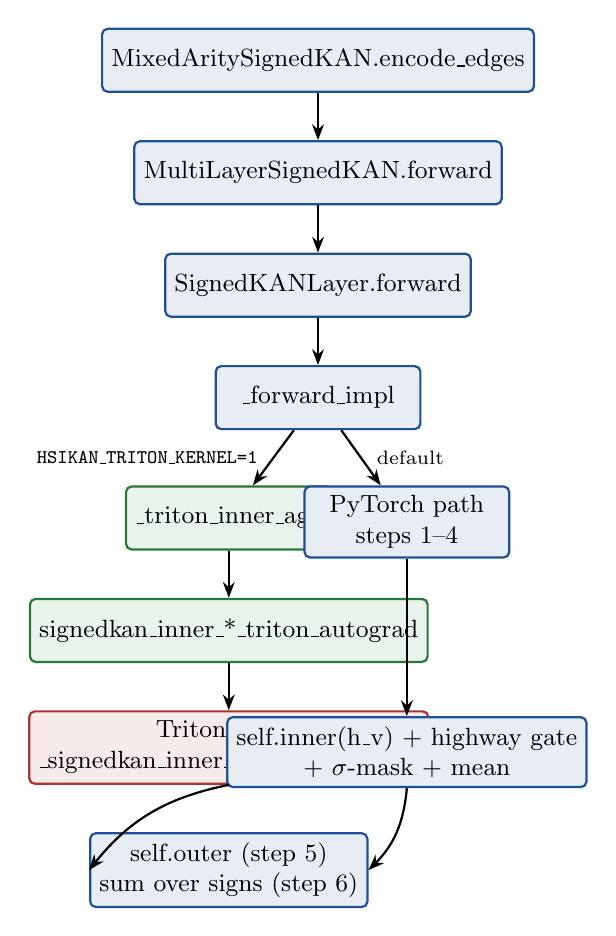
\begin{tikzpicture}[node distance=0.6cm and 0.5cm]
  \node[bluebox] (a)  {MixedAritySignedKAN.encode\_edges};
  \node[bluebox, below=of a] (b) {MultiLayerSignedKAN.forward};
  \node[bluebox, below=of b] (c) {SignedKANLayer.forward};
  \node[bluebox, below=of c] (d) {\_forward\_impl};
  \node[greenbox, below left=0.7cm and -1.5cm of d] (e) {\_triton\_inner\_agg};
  \node[bluebox, below right=0.7cm and -1.5cm of d] (f) {PyTorch path \\ steps 1--4};
  \node[greenbox, below=of e] (g) {signedkan\_inner\_*\_triton\_autograd};
  \node[redbox, below=of g] (i) {Triton kernel \\ \_signedkan\_inner\_(highway\_)kernel};
  \node[bluebox, below=2cm of f] (k) {self.inner(h\_v) + highway gate \\ + $\sigma$-mask + mean};
  \node[bluebox, below=of i] (l) {self.outer (step 5) \\ sum over signs (step 6)};

  \draw[arrow] (a) -- (b);
  \draw[arrow] (b) -- (c);
  \draw[arrow] (c) -- (d);
  \draw[arrow] (d) -- node[left,xshift=-2pt,font=\scriptsize]{\texttt{HSIKAN\_TRITON\_KERNEL=1}} (e);
  \draw[arrow] (d) -- node[right,xshift=2pt,font=\scriptsize]{default} (f);
  \draw[arrow] (e) -- (g);
  \draw[arrow] (g) -- (i);
  \draw[arrow] (f) -- (k);
  \draw[arrow] (i.south) to[bend right=20] (l.west);
  \draw[arrow] (k.south) to[bend left=20]  (l.east);
\end{tikzpicture}
\end{center}

The kernel covers steps 1--4 of \texttt{\_forward\_impl} (gather, per-sign CR, highway-skip, $\sigma$-mask, mean reduce). Steps 5--6 (outer spline + sum-over-signs) stay in PyTorch --- they are already cheap.

% ─── §3 ─────────────────────────────────────────────────────────────
\section{Build process — six steps, in order}

\begin{center}
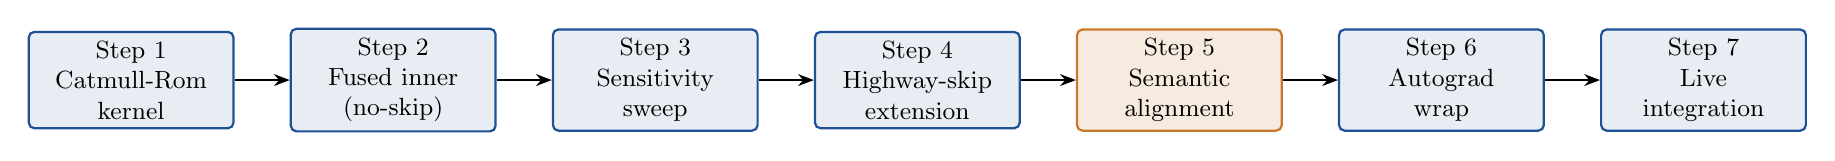
\begin{tikzpicture}[node distance=0.4cm and 0.7cm]
  \node[bluebox]                 (s1) {Step 1\\Catmull-Rom\\kernel};
  \node[bluebox, right=of s1]    (s2) {Step 2\\Fused inner\\(no-skip)};
  \node[bluebox, right=of s2]    (s3) {Step 3\\Sensitivity\\sweep};
  \node[bluebox, right=of s3]    (s4) {Step 4\\Highway-skip\\extension};
  \node[warnbox, right=of s4]    (s5) {Step 5\\Semantic\\alignment};
  \node[bluebox, right=of s5]    (s6) {Step 6\\Autograd\\wrap};
  \node[bluebox, right=of s6]    (s7) {Step 7\\Live\\integration};

  \draw[arrow] (s1) -- (s2);
  \draw[arrow] (s2) -- (s3);
  \draw[arrow] (s3) -- (s4);
  \draw[arrow] (s4) -- (s5);
  \draw[arrow] (s5) -- (s6);
  \draw[arrow] (s6) -- (s7);
\end{tikzpicture}
\end{center}

\paragraph{Step 1 — Catmull-Rom kernel.}
Port \texttt{\_catmull\_rom\_eval} (the leaf operation) first. It is the simplest unit and validates the basic Triton plumbing.
\textit{Acceptance:} forward parity $\le 10^{-4}$ vs reference at 6 shapes; speedup $\ge 5\times$ at canonical shape.

\paragraph{Step 2 — Fused inner (no-skip).}
Fuse the gather + per-sign CR + $\sigma$-mask + mean reduce into one kernel. This is where the real speedup lives --- it eliminates the $(T, k, 2, d)$ intermediate that the PyTorch path materialises.
\textit{Acceptance:} forward parity $\le 10^{-4}$; speedup $\ge 10\times$ at canonical shape; arity-agnostic over $k=2{\dots}6$.

\paragraph{Step 3 — Sensitivity sweep.}
Map the kernel's performance landscape across $(T, d, k, G, \mathrm{BLOCK\_T}, \mathrm{BLOCK\_D})$. Don't skip this: block-size defaults can cost $2\times$ speedup. We found $\mathrm{BLOCK\_T}=16$ was $2\times$ faster than the default $32$ at $d=4$ --- pure default-tuning win.

\paragraph{Step 4 — Skip-variant extension.}
Most production paths have an inner skip (residual / highway). Inline a $d$-by-$d$ matvec for the gate logit:
\(
\ell_{c} = \sum_{e=0}^{d-1} W_{e,c} \cdot h_{e} + b_{c}
\),
costing $O(d^2)$ extra work per $(t, k, d_c)$ but the gather + CR remain dominant for $d \le 32$.

\paragraph{Step 5 — Semantic alignment with production. \textbf{(Critical.)}}
This is the step that catches bugs before they regress live training. Run a parity test against the \emph{actual production layer}, not against your own test reference (which may differ from production).

\begin{center}
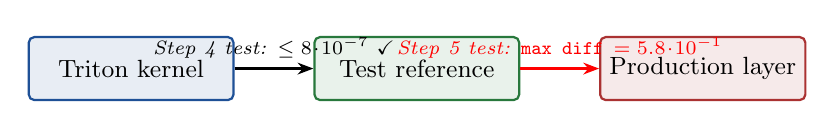
\begin{tikzpicture}[node distance=0.4cm and 1cm]
  \node[bluebox]                  (T)  {Triton kernel};
  \node[greenbox, right=of T]     (TR) {Test reference};
  \node[redbox, right=of TR]      (PR) {Production layer};
  \draw[arrow] (T) -- node[above,font=\scriptsize]{\textit{Step 4 test:} $\le 8\!\cdot\!10^{-7}$ \checkmark} (TR);
  \draw[arrow,red] (TR) -- node[above,font=\scriptsize]{\textit{Step 5 test:} \texttt{max diff $=5.8\!\cdot\!10^{-1}$}} (PR);
\end{tikzpicture}
\end{center}

In our case, the kernel applied $\tanh(\mathrm{CR}(x))$ and used a clamped-$h_v$ residual. Production \texttt{SignedKANLayer.\_forward\_impl} did \emph{neither} --- raw CR output, raw $h_v$ residual. The fix:

\begin{itemize}[leftmargin=*]
  \item Drop \texttt{tl.extra.libdevice.tanh(cr)} $\to$ just \texttt{cr} in both kernels.
  \item Replace \texttt{x\_clamp} $\to$ \texttt{x} in the highway residual term.
  \item Update the PyTorch reference in tests + sensitivity + autograd backward to match.
\end{itemize}

After fix: parity vs production layer $= 1.2\cdot 10^{-7}$ highway, $9.9\cdot 10^{-8}$ no-skip.

\paragraph{Step 6 — Autograd wrap.}
The kernel returns a tensor without an autograd graph. Wrap each variant in a \texttt{torch.autograd.Function}. Forward calls the Triton kernel; backward (v0) re-runs the forward through the PyTorch reference under autograd. Slower than a fused backward but correct without writing one.
\textit{Acceptance:} $\partial x, \partial \mathrm{coef}_{\pm}, \partial W, \partial b$ all match reference to $\le 10^{-4}$.

\paragraph{Step 7 — Live integration with env-gating.}
Add a fast-path in \texttt{\_forward\_impl} that dispatches to the autograd-wrapped kernel when conditions match. \textbf{Gate the dispatch behind an env var, default OFF}, until the backward kernel matches the forward path's memory profile.

\begin{lstlisting}
def _can_use_triton_inner(self, x):
    if int(os.environ.get("HSIKAN_TRITON_KERNEL", "0")) == 0:
        return False
    if not x.is_cuda: return False
    if self.n_branches != 2: return False
    if self.inner_skip not in ("none", "highway"): return False
    if not isinstance(self.inner, BatchedCatmullRomActivation):
        return False
    try: import triton  # noqa
    except ImportError: return False
    return True
\end{lstlisting}

% ─── §4 ─────────────────────────────────────────────────────────────
\section{Test tiers}

\begin{center}
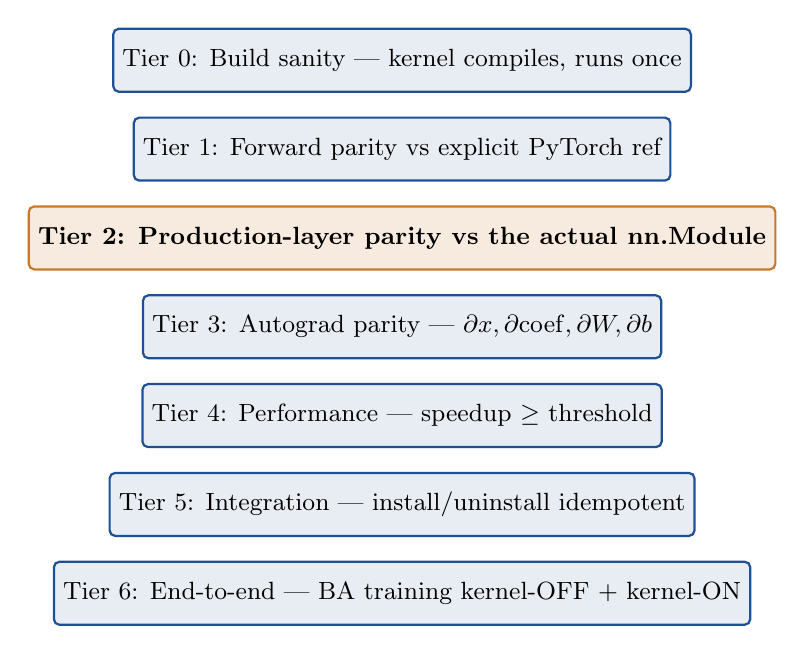
\begin{tikzpicture}[node distance=0.3cm]
  \node[bluebox]                  (T0) {Tier 0: Build sanity --- kernel compiles, runs once};
  \node[bluebox, below=of T0]     (T1) {Tier 1: Forward parity vs explicit PyTorch ref};
  \node[warnbox, below=of T1]     (T2) {\textbf{Tier 2: Production-layer parity vs the actual nn.Module}};
  \node[bluebox, below=of T2]     (T3) {Tier 3: Autograd parity --- $\partial x, \partial \mathrm{coef}, \partial W, \partial b$};
  \node[bluebox, below=of T3]     (T4) {Tier 4: Performance --- speedup $\ge$ threshold};
  \node[bluebox, below=of T4]     (T5) {Tier 5: Integration --- install/uninstall idempotent};
  \node[bluebox, below=of T5]     (T6) {Tier 6: End-to-end --- BA training kernel-OFF + kernel-ON};
\end{tikzpicture}
\end{center}

\begin{center}
\begin{tabular}{c p{0.78\linewidth}}
\toprule
\textbf{tier} & \textbf{what passes} \\
\midrule
0  & kernel returns expected-shape tensor; no compile error \\
1  & $|\,\text{out}_\text{kernel} - \text{out}_\text{ref}\,|_{\max} < 10^{-4}$ at $\ge 3$ shapes \\
2  & \textbf{parity vs the production \texttt{SignedKANLayer.forward} (or whatever the production caller is)} $\le 10^{-4}$ \\
3  & gradient parity $\le 10^{-4}$ for every differentiable input \\
4  & speedup $\ge 5\times$ (CR), $\ge 10\times$ (fused inner) at canonical shape \\
5  & install + uninstall is a semantic no-op; idempotent under repeated calls \\
6  & BA training with \texttt{HSIKAN\_TRITON\_KERNEL=0/1} produces comparable AUC ($\pm 1\%$); kernel-OFF run does not OOM \\
\bottomrule
\end{tabular}
\end{center}

The current suite has 31 tests covering tiers 1, 3, 4, 5, 6. \textbf{Tier 2 was missing in the first pass} --- that's how the semantic divergence shipped to integration before being caught.

% ─── §5 ─────────────────────────────────────────────────────────────
\section{The math — forward and backward in closed form}

This section gives the kernel's exact forward function and the closed-form gradients the fused backward kernel needs to compute.

\paragraph{Notation.}
$V$ = number of vertices, $T$ = number of cycles, $k$ = arity, $d$ = hidden dim, $G$ = grid (control-point count), $S=2$ = sign branches.
$x \in \mathbb{R}^{V\times d}$ (vertex embeddings),
$v \in \{0,\dots,V-1\}^{T\times k}$ (\texttt{triad\_v}),
$\sigma \in \{+1,-1\}^{T\times k}$ (\texttt{triad\_sigma}),
$C^{+}, C^{-} \in \mathbb{R}^{d\times G}$ (\texttt{coef\_pos}, \texttt{coef\_neg}),
$W \in \mathbb{R}^{d\times d}$, $b \in \mathbb{R}^{d}$ (\texttt{gate\_w}, \texttt{gate\_b}),
$\mathrm{agg} \in \mathbb{R}^{T\times S\times d}$ (kernel output).

\subsection{Forward (Highway variant, matches production)}

For each cycle $t \in [T]$, slot $i \in [k]$, channel $c \in [d]$:
\[
h_{t,i,c} = x_{v_{t,i},\,c}, \qquad
\hat h_{t,i,c} = \mathrm{clamp}(h_{t,i,c}, -1, 1).
\]

\paragraph{Catmull-Rom evaluation.}
Let $u = (\hat h + 1) \cdot \tfrac{G-1}{2}$, $j = \lfloor u \rfloor$, $\tau = u - j$. The four blending weights are
\begin{align*}
w_{-1}(\tau) &= \tfrac{1}{2}(-\tau^3 + 2\tau^2 - \tau), &
w_{0}(\tau)  &= \tfrac{1}{2}(3\tau^3 - 5\tau^2 + 2),\\
w_{+1}(\tau) &= \tfrac{1}{2}(-3\tau^3 + 4\tau^2 + \tau), &
w_{+2}(\tau) &= \tfrac{1}{2}(\tau^3 - \tau^2),
\end{align*}
so for sign $s \in \{+,-\}$:
\[
\mathrm{CR}^{s}_{t,i,c}
 = \sum_{p \in \{-1,0,+1,+2\}} w_p(\tau_{t,i,c}) \cdot
   C^{s}_{c,\,\mathrm{clip}(j_{t,i,c}+p,\,0,\,G-1)}.
\]

\paragraph{Highway gate.}
Per-$(t,i,c)$ sigmoid of a $d$-by-$d$ matvec:
\[
\ell_{t,i,c} = \sum_{e=0}^{d-1} W_{e,c} \cdot h_{t,i,e} + b_c,
\qquad
T_{t,i,c} = \sigma(\ell_{t,i,c}) = \frac{1}{1 + e^{-\ell_{t,i,c}}}.
\]

\paragraph{Highway mix.}
Raw $h$ residual --- production semantics, no \texttt{tanh} wrap:
\[
H^{s}_{t,i,c} = T_{t,i,c} \cdot \mathrm{CR}^{s}_{t,i,c}
              + (1 - T_{t,i,c}) \cdot h_{t,i,c}.
\]

\paragraph{$\sigma$-masked mean.}
\[
m^{s}_{t,i} = \mathbb{1}[\sigma_{t,i} = s], \quad
n^{s}_{t} = \max\!\Big(1,\, \sum_{i} m^{s}_{t,i}\Big),
\]
\[
\boxed{\;
\mathrm{agg}^{s}_{t,c} \;=\; \frac{1}{n^{s}_{t}} \sum_{i=0}^{k-1} m^{s}_{t,i} \cdot H^{s}_{t,i,c}.
\;}
\]
The no-skip variant drops the gate: $H^{s}_{t,i,c} \mapsto \mathrm{CR}^{s}_{t,i,c}$.

\subsection{Backward — what the fused backward kernel must compute}

Given the upstream gradient $g^{s}_{t,c} = \partial \mathcal{L} / \partial \mathrm{agg}^{s}_{t,c}$, the backward outputs five gradients: $\partial\mathcal{L}/\partial x$, $\partial\mathcal{L}/\partial C^{+}$, $\partial\mathcal{L}/\partial C^{-}$, $\partial\mathcal{L}/\partial W$, $\partial\mathcal{L}/\partial b$.

\paragraph{Per-cycle-slot pre-gradient} (broadcast over masked slots, divide by count):
\[
\tilde g^{s}_{t,i,c} \;=\; \frac{m^{s}_{t,i}}{n^{s}_{t}} \cdot g^{s}_{t,c}.
\]
This is the only $(T \times k \times S \times d)$ tensor the backward needs --- and it can be streamed inside the kernel without materialising it.

\paragraph{Highway-gate locals} (pre-computed once per $(t,i,c)$):
\[
\Delta^{s}_{t,i,c} = \mathrm{CR}^{s}_{t,i,c} - h_{t,i,c},
\qquad
\partial T / \partial \ell = T(1-T).
\]

\subsubsection{(a) $\partial \mathcal{L} / \partial x$ — three contributions}

Three additive paths from $\mathrm{agg}$ back to $x$:
\begin{description}[leftmargin=2em,style=nextline]
\item[(i) Residual path]
\(\displaystyle
\frac{\partial \mathrm{agg}^{s}_{t,c}}{\partial h_{t,i,c}}\bigg|_{\text{res}}
= \frac{m^{s}_{t,i}}{n^{s}_{t}} (1 - T_{t,i,c}).
\)
\item[(ii) Gate-logit path] (the gate uses \emph{all} $d$ components of $h_{t,i}$, so $\partial \mathrm{agg}_{c}/\partial h_{e} \neq 0$ for $e \neq c$):
\(\displaystyle
\frac{\partial \mathrm{agg}^{s}_{t,c}}{\partial h_{t,i,e}}\bigg|_{\text{gate}}
= \frac{m^{s}_{t,i}}{n^{s}_{t}} \cdot \Delta^{s}_{t,i,c} \cdot T_{t,i,c}(1 - T_{t,i,c}) \cdot W_{e,c}.
\)
\item[(iii) Spline-input path]
\(\displaystyle
\frac{\partial \mathrm{agg}^{s}_{t,c}}{\partial h_{t,i,c}}\bigg|_{\text{CR}}
= \frac{m^{s}_{t,i}}{n^{s}_{t}} \cdot T_{t,i,c} \cdot \frac{\partial \mathrm{CR}^{s}_{t,i,c}}{\partial h_{t,i,c}},
\)
\end{description}
with $\partial \mathrm{CR}^{s}_{t,i,c} / \partial h_{t,i,c}$ from the CR closed form (zero on \texttt{clamp}-saturated inputs):
\[
\frac{\partial \mathrm{CR}^{s}_{t,i,c}}{\partial h_{t,i,c}}
= \mathbb{1}[|h_{t,i,c}| < 1] \cdot \frac{G-1}{2} \sum_{p} w'_p(\tau_{t,i,c}) \cdot C^{s}_{c,\,\mathrm{clip}(j+p)},
\]
where $w'_{-1}(\tau) = \tfrac{1}{2}(-3\tau^2+4\tau-1)$, $w'_{0}(\tau) = \tfrac{1}{2}(9\tau^2-10\tau)$, $w'_{+1}(\tau) = \tfrac{1}{2}(-9\tau^2+8\tau+1)$, $w'_{+2}(\tau) = \tfrac{1}{2}(3\tau^2-2\tau)$.

The kernel scatter-adds the three paths into $\partial\mathcal{L}/\partial x$ at vertex index $v_{t,i}$:
\[
\frac{\partial \mathcal{L}}{\partial x_{v,e}} = \!\!\!\sum_{(t,i)\,:\,v_{t,i}=v} \sum_{s} \tilde g^{s}_{t,i,c}
\cdot \big[(1{-}T)_{t,i,e}\,\delta_{e,c} + \Delta^{s}_{t,i,c}\,T(1{-}T)_{t,i,c}\,W_{e,c} + T_{t,i,e}\,\partial \mathrm{CR}/\partial h_{t,i,e}\,\delta_{e,c}\big].
\]

\subsubsection{(b) $\partial \mathcal{L} / \partial C^{+}, \partial \mathcal{L} / \partial C^{-}$ — control-point gradients}

The CR output is \emph{linear} in the control points, so
\[
\frac{\partial \mathrm{CR}^{s}_{t,i,c}}{\partial C^{s}_{c, q}}
= \sum_{p \in \{-1,0,+1,+2\}} w_p(\tau_{t,i,c}) \cdot
\mathbb{1}\!\left[\mathrm{clip}(j_{t,i,c}+p,\,0,\,G-1) = q\right].
\]
Scatter-add over $(t, i)$:
\[
\boxed{\;
\frac{\partial \mathcal{L}}{\partial C^{s}_{c, q}}
= \sum_{t,i} \tilde g^{s}_{t,i,c} \cdot T_{t,i,c} \cdot
\sum_{p} w_p(\tau_{t,i,c}) \cdot \mathbb{1}\!\left[\mathrm{clip}(j+p) = q\right].
\;}
\]
Only sign-$s$ slots contribute (via $m^{s}_{t,i}$ in $\tilde g^{s}$).

\subsubsection{(c) $\partial \mathcal{L} / \partial W, \partial \mathcal{L} / \partial b$ — gate Linear gradients}

\[
\frac{\partial \mathcal{L}}{\partial W_{e, c}}
= \sum_{s, t, i} \tilde g^{s}_{t,i,c} \cdot \Delta^{s}_{t,i,c} \cdot T_{t,i,c}(1 - T_{t,i,c}) \cdot h_{t,i,e},
\]
\[
\frac{\partial \mathcal{L}}{\partial b_{c}}
= \sum_{s, t, i} \tilde g^{s}_{t,i,c} \cdot \Delta^{s}_{t,i,c} \cdot T_{t,i,c}(1 - T_{t,i,c}).
\]
Both are reductions over $(s, t, i)$ --- no scatter, just an accumulator-per-$(e,c)$ or per-$(c)$ in registers, atomic-add-flushed at block end.

\subsection{Memory profile of the fused backward}

The PyTorch-ref backward (current v0) materialises the $(T, k, S, d)$ post-highway intermediate inside the autograd graph. At Slashdot scale ($T=200\text{K}$, $k=4$, $S=2$, $d=4$) that is $\sim 25\,\text{MB}$ per layer; across multiple layers + autograd-retained inputs the peak hits $\sim 6\,\text{GiB}$ on BA-scale runs.

The fused backward kernel's working set per program block is $O(\mathrm{BLOCK\_T} \cdot d \cdot k)$ --- under $1\,\text{MB}$ at canonical block sizes. The only $O(T \cdot k \cdot d)$ allocation is \texttt{agg\_grad\_in} (the upstream $g$, just the kernel input), and the only $O(T \cdot d)$ write is \texttt{x\_grad\_out} via scatter-add.

\textbf{Predicted memory for the fused backward at Slashdot SOTA shape: $\sim 30\,\text{MB}$ peak} (vs $6\,\text{GiB}$ for the v0 ref). That is the gap that has to close before live integration can be enabled at training time on $8\,\text{GiB}$ GPUs.

% ─── §6 ─────────────────────────────────────────────────────────────
\section{Forward-semantics comparison: before vs after the fix}

\begin{center}
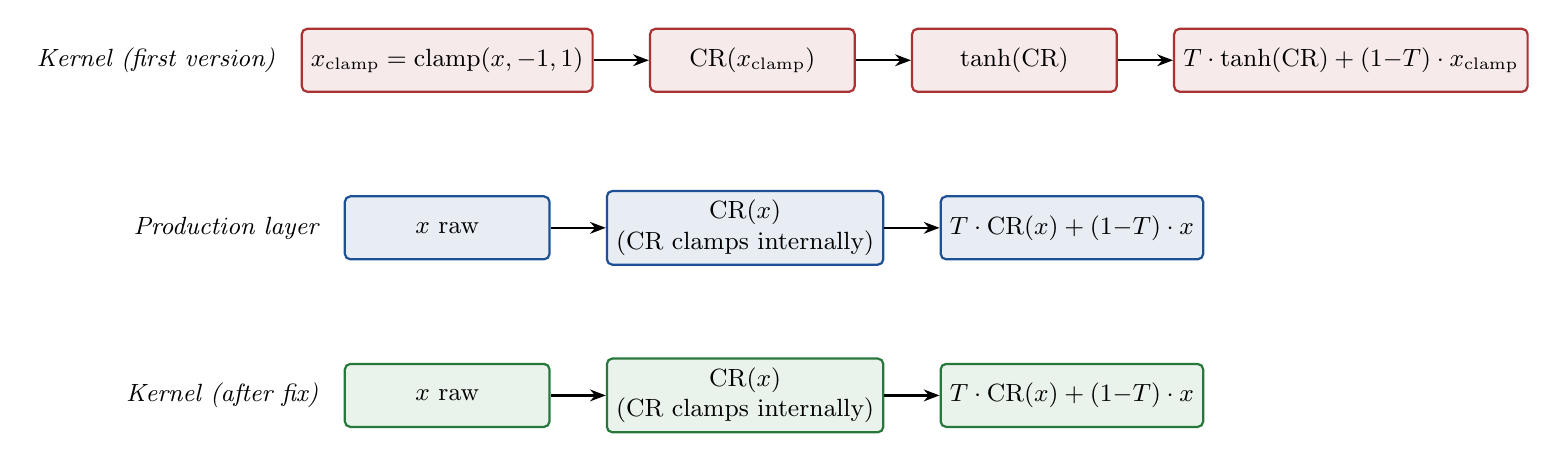
\begin{tikzpicture}[node distance=0.5cm and 0.7cm]
  % Before
  \node[redbox]   (B1) {$x_{\text{clamp}} = \mathrm{clamp}(x,-1,1)$};
  \node[redbox, right=of B1] (B2) {$\mathrm{CR}(x_{\text{clamp}})$};
  \node[redbox, right=of B2] (B3) {$\tanh(\mathrm{CR})$};
  \node[redbox, right=of B3] (B4) {$T \cdot \tanh(\mathrm{CR}) + (1{-}T) \cdot x_{\text{clamp}}$};
  \node[left=0.2cm of B1, font=\small\itshape] {Kernel (first version)};

  \draw[arrow] (B1) -- (B2);
  \draw[arrow] (B2) -- (B3);
  \draw[arrow] (B3) -- (B4);

  % Production
  \node[bluebox, below=1.3cm of B1] (P1) {$x$ raw};
  \node[bluebox, right=of P1] (P2) {$\mathrm{CR}(x)$ \\ (CR clamps internally)};
  \node[bluebox, right=of P2] (P3) {$T \cdot \mathrm{CR}(x) + (1{-}T) \cdot x$};
  \node[left=0.2cm of P1, font=\small\itshape] {Production layer};

  \draw[arrow] (P1) -- (P2);
  \draw[arrow] (P2) -- (P3);

  % After
  \node[greenbox, below=1.3cm of P1] (A1) {$x$ raw};
  \node[greenbox, right=of A1] (A2) {$\mathrm{CR}(x)$ \\ (CR clamps internally)};
  \node[greenbox, right=of A2] (A3) {$T \cdot \mathrm{CR}(x) + (1{-}T) \cdot x$};
  \node[left=0.2cm of A1, font=\small\itshape] {Kernel (after fix)};

  \draw[arrow] (A1) -- (A2);
  \draw[arrow] (A2) -- (A3);
\end{tikzpicture}
\end{center}

The kernel's first version applied two semantic transforms that production never did. Both came from a misread of the original PyTorch path. The fix is two characters of Triton (drop \texttt{tanh}) and one rename ($x_{\text{clamp}} \to x$) --- but you have to \emph{see} the divergence first, which requires Tier-2 testing.

% ─── §7 ─────────────────────────────────────────────────────────────
\section{The OOM trap and why integration is env-gated}

\begin{center}
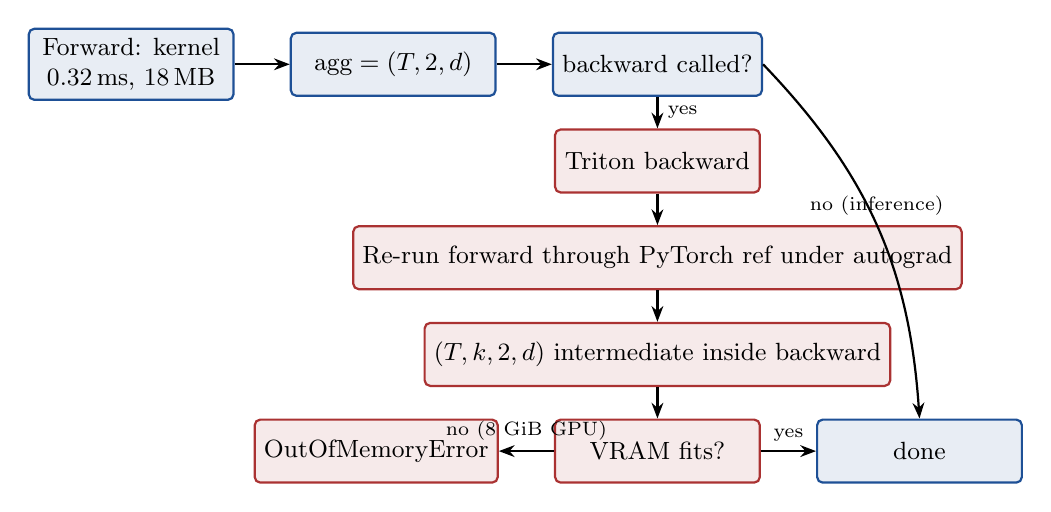
\begin{tikzpicture}[node distance=0.4cm and 0.7cm]
  \node[bluebox]                  (A) {Forward: kernel\\$0.32\,\text{ms}$, $18\,\text{MB}$};
  \node[bluebox, right=of A]      (B) {$\text{agg} = (T,2,d)$};
  \node[bluebox, right=of B]      (C) {backward called?};
  \node[redbox, below=of C]       (D) {Triton backward};
  \node[redbox, below=of D]       (E) {Re-run forward through PyTorch ref under autograd};
  \node[redbox, below=of E]       (F) {$(T, k, 2, d)$ intermediate inside backward};
  \node[redbox, below=of F]       (G) {VRAM fits?};
  \node[redbox, left=of G]        (H) {OutOfMemoryError};
  \node[bluebox, right=of G]      (Z) {done};

  \draw[arrow] (A) -- (B);
  \draw[arrow] (B) -- (C);
  \draw[arrow] (C) -- node[right,font=\scriptsize]{yes} (D);
  \draw[arrow] (C.east) to[bend left=20] node[above,font=\scriptsize]{no (inference)} (Z.north);
  \draw[arrow] (D) -- (E);
  \draw[arrow] (E) -- (F);
  \draw[arrow] (F) -- (G);
  \draw[arrow] (G) -- node[above,font=\scriptsize]{no (8 GiB GPU)} (H);
  \draw[arrow] (G) -- node[above,font=\scriptsize]{yes} (Z);
\end{tikzpicture}
\end{center}

The Triton autograd \texttt{forward} is fast and memory-light --- but the \textbf{\texttt{backward} is a PyTorch re-compute}. It allocates the very intermediate the kernel was supposed to avoid. On the BA end-to-end test ($T \sim 50\text{K}$, $k=4$, $d=8$, multiple layers), that intermediate hits $6\,\text{GiB}$ and OOMs an $8\,\text{GiB}$ GPU.

\textbf{This is why live integration is env-gated, default OFF.} The kernel is ready for forward-only / inference paths today; training-time enabling requires the fused backward kernel.

% ─── §8 ─────────────────────────────────────────────────────────────
\section{Common pitfalls — checklist}

\begin{itemize}[leftmargin=2em]
  \item[$\square$] \textbf{Step 5 / Tier 2 — production parity, not test-ref parity.} The most expensive bug we shipped. Always include a parity test against the actual nn.Module the kernel is replacing.
  \item[$\square$] \textbf{BLOCK\_T default.} Start at the next power of 2 above your typical batch dimension and sweep down to 8. We found 16 was $2\times$ faster than 32 at $d=4$.
  \item[$\square$] \textbf{CR domain clamping.} The CR spline only supports $x \in [-1, 1]$. Production \texttt{\_catmull\_rom\_eval} clamps internally; if your kernel does too, make sure the residual term uses raw $x$, not the clamped one.
  \item[$\square$] \textbf{Backward memory.} A correct-but-slow PyTorch-ref backward can OOM at training scale even when the forward is fine. Plan the backward kernel before claiming integration is done.
  \item[$\square$] \textbf{Autograd wrapping.} A bare Triton call returns a tensor without a graph --- \texttt{loss.backward()} will silently miss it. Wrap in \texttt{torch.autograd.Function}.
  \item[$\square$] \textbf{Env-gate the integration} until the full forward+backward path is safe at production scale. Default OFF.
  \item[$\square$] \textbf{Speedup numbers are PyTorch-ref-relative.} When you change the reference (e.g.\ drop \texttt{tanh}), the speedup number changes too --- not because the kernel got slower but because the baseline got faster.
\end{itemize}

% ─── §9 ─────────────────────────────────────────────────────────────
\section{Files of record}

\begin{center}
\begin{tabular}{p{0.45\linewidth} p{0.5\linewidth}}
\toprule
\textbf{file} & \textbf{role} \\
\midrule
\texttt{signedkan\_wip/src/triton\_kernels.py}              & kernels, autograd wrappers, install/uninstall \\
\texttt{signedkan\_wip/src/triton\_kernels\_sensitivity.py} & parameter sensitivity sweep \\
\texttt{signedkan\_wip/tests/test\_triton\_kernels.py}      & 31 tests, tiers 1/3/4/5/6 \\
\texttt{signedkan\_wip/src/signedkan.py}                    & live integration fast-path \\
\texttt{docs/triton\_kernel\_integration\_tutorial\_2026\_05\_09.md} & this document (markdown) \\
\texttt{reports/triton\_kernel\_integration\_tutorial\_2026\_05\_09.tex} & this document (\LaTeX{}) \\
\bottomrule
\end{tabular}
\end{center}

% ─── §10 ─────────────────────────────────────────────────────────────
\section{Quick reference — running the suite}

\begin{lstlisting}[language=bash]
# Full suite (<= 60s)
python -m pytest signedkan_wip/tests/test_triton_kernels.py -v

# Skip the slow end-to-end BA training test (<= 5s)
python -m pytest signedkan_wip/tests/test_triton_kernels.py -v -k "not end_to_end_ba"

# Sensitivity sweep (~2 min)
python -m signedkan_wip.src.triton_kernels_sensitivity

# Try training with the kernel ON
# (forward-only OK; backward may OOM on small GPUs until fused-backward lands)
HSIKAN_TRITON_KERNEL=1 python -m signedkan_wip.src.run_final_cell --dataset bitcoin_alpha
\end{lstlisting}

\end{document}
